\section{Training Dynamics}
In this section, we analyze the training dynamics. As shown in Figure~\ref{fig:training-dynamics}, multi-turn RL for kernel generation exhibits significant instability, characterized by elevated entropy, perplexity, and gradient norms, even when using unbiased advantage estimation. Incorporating mismatch correction (i.e., Mismatch Rejection Sampling) effectively stabilizes the training process. Furthermore, the introduction of PR and PRS provides additional stability, leading to smoother training.
\begin{figure*}[htbp]
  \centering
  % Row 1
  \begin{minipage}[t]{0.49\textwidth}
    \centering
    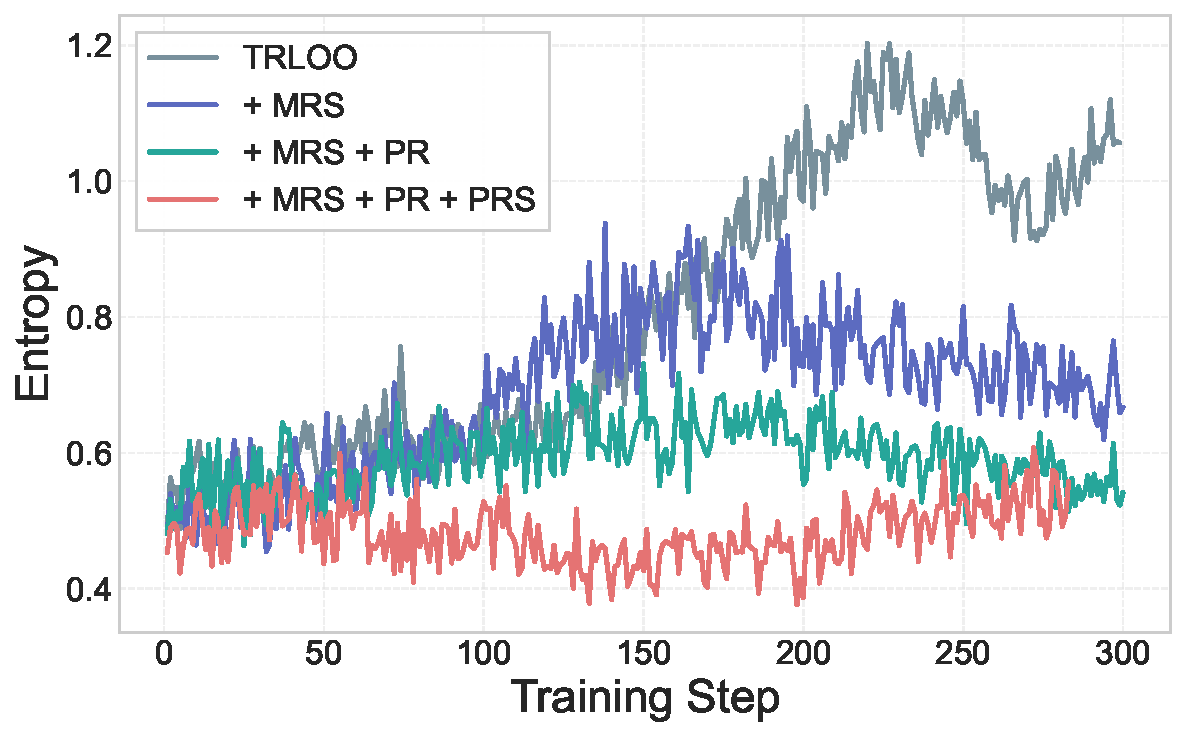
\includegraphics[width=\linewidth]{figures/entropy.pdf} % TODO
  \end{minipage}
  \hfill
  \begin{minipage}[t]{0.49\textwidth}
    \centering
    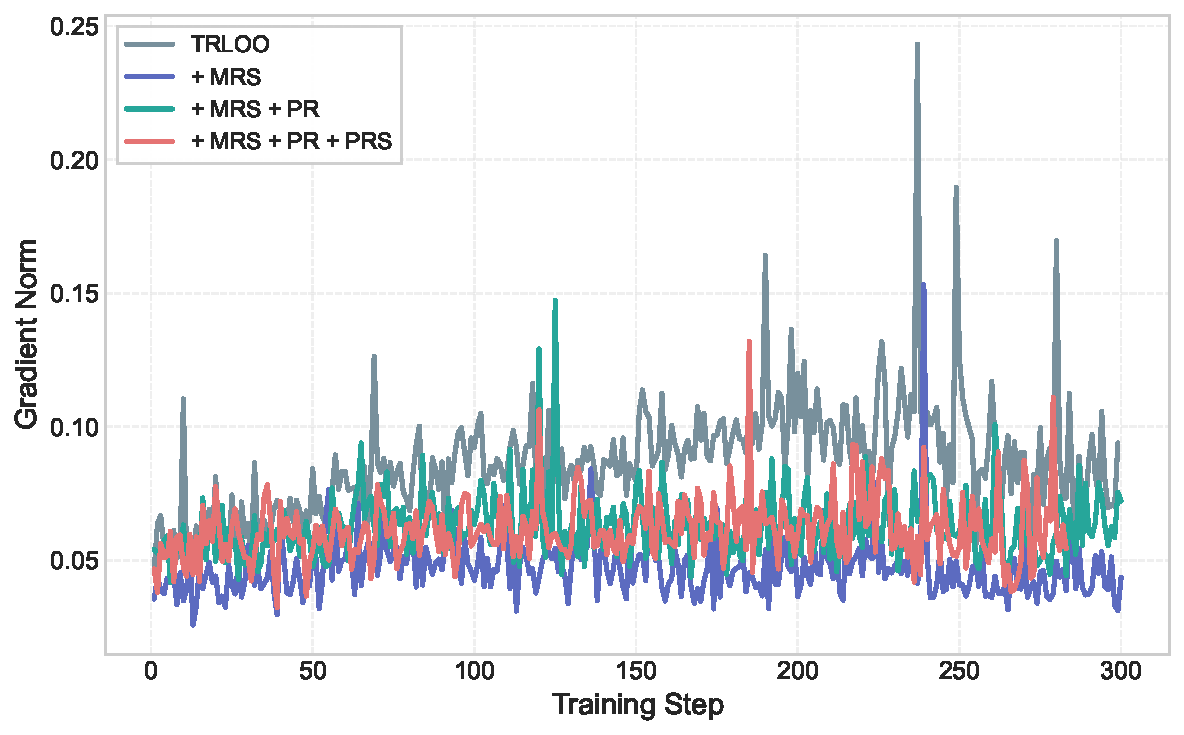
\includegraphics[width=\linewidth]{figures/grad-norm.pdf} % TODO
  \end{minipage}

  \vspace{0.6em} % adjust vertical gap between rows

  % Row 2
  \begin{minipage}[t]{0.49\textwidth}
    \centering
    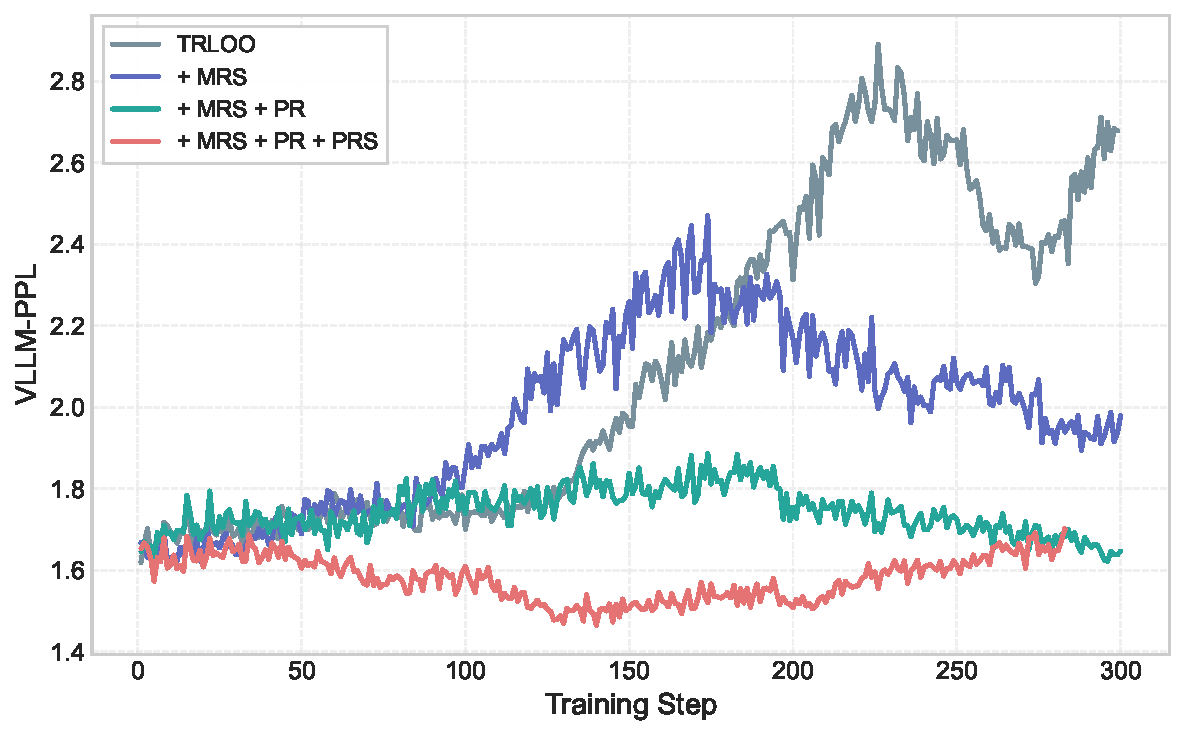
\includegraphics[width=\linewidth]{figures/vllm-ppl.pdf} % TODO
  \end{minipage}
  \hfill
  \begin{minipage}[t]{0.49\textwidth}
    \centering
    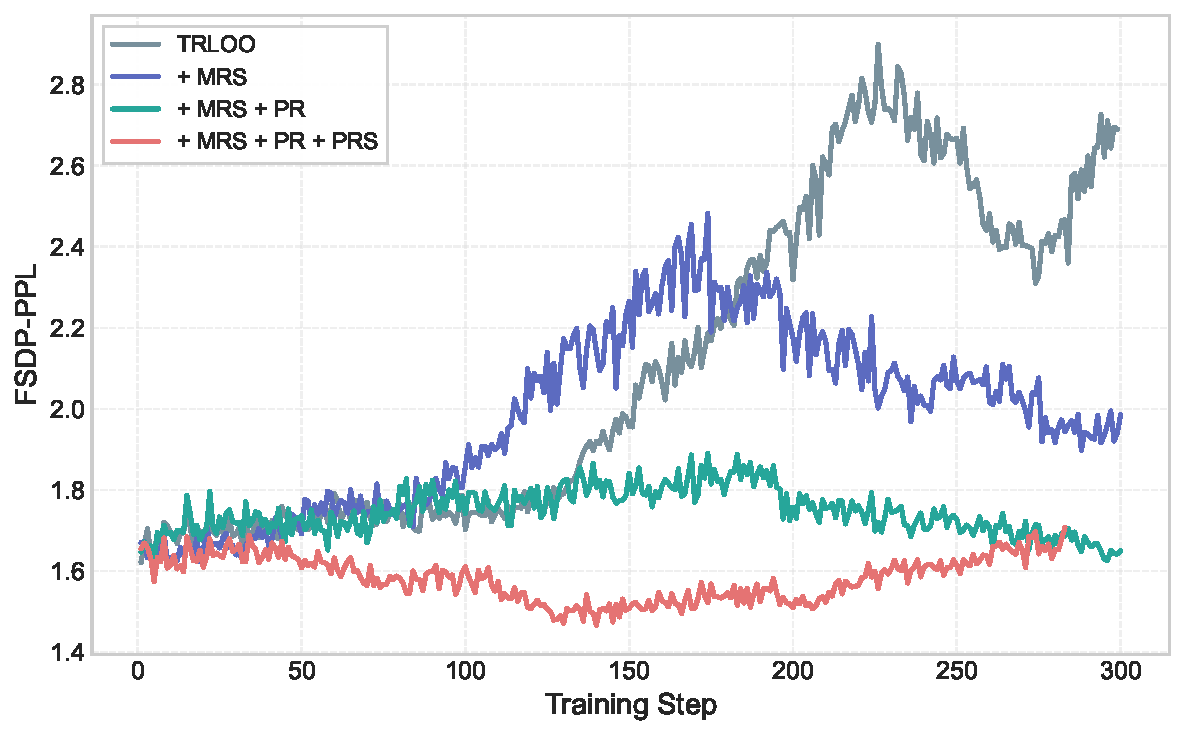
\includegraphics[width=\linewidth]{figures/fsdp-ppl.pdf} % TODO
  \end{minipage}

  \caption{The training dynamics of TRLOO, TRLOO + Mismatch Rejection Sampling (MRS), TRLOO + MRS + Profiling-based Reward (PR) and TRLOO + MRS + PR + Profiling-based Rejection Sampling (PRS). We analyze the training dynamics via the lens of entropy, gradient norm, VLLM-PPL, and FSDP-PPL, which are also monitored by ~\citet{liu-li-2025-rl-collapse}.}
  \label{fig:training-dynamics}
\end{figure*}
